\documentclass[12pt]{scrartcl}
\usepackage{tocbasic}
\RedeclareSectionCommand[tocindent=0pt]{section}
\usepackage{scrlayer-scrpage} 					% Package for header and footer
\usepackage[reqno]{amsmath} 				    % Additional mathematical constructs
\usepackage{amsfonts} 							% Mathematical fonts
\usepackage[utf8]{inputenc}						% Text in UTF-8 character set
%\usepackage[ngerman]{babel} 					% German hyphenation
\usepackage[T1]{fontenc}						% Umlauts as separate characters
\usepackage{textcomp}							% TS1-encoding symbols
\usepackage{txfonts}							% Font: Times New Roman
\usepackage{lipsum}								% Package to generate dummy text for testing the source code
%%%%%%%%%%%%%%%%%%%%%%%
%Bibliography
%%%%%%%%%%%%%%%%%%%%%%%
%\usepackage[style=german,german=quotes]{csquotes}	% Package for citations and bibliography
\usepackage[backend=bibtex, style=authoryear,sorting=nyt,url=false, doi=false, isbn=false ,eprint=false,maxnames=3,maxbibnames=99]{biblatex} 
\renewbibmacro*{publisher+location+date}{%
	\printlist{publisher}%
	\iflistundef{location}
	{\setunit*{\addcomma\space}}
	{\setunit*{\addcomma\space}}%
	\printlist{location}%
	\setunit*{\addcomma\space}%
	\usebibmacro{date}%
	\newunit}
\renewbibmacro*{byeditor+others}{% %Hg. or Hgg. in parentheses after editor, instead of before
	\ifnameundef{editor}
	{}
	{\printnames[byeditor]{editor}%
		\setunit{\addspace}%
		\usebibmacro{editor+othersstrg}%
		\clearname{editor}%
		\newunit}%
	\usebibmacro{byeditorx}%
	\usebibmacro{bytranslator+others}} 
\DeclareFieldFormat{editortype}{\mkbibparens{#1}}
\DefineBibliographyStrings{german}{byeditor = {\mkbibparens{Ed\adddot}}}   
\DeclareFieldFormat[incollection]{pages}{#1}%
\DeclareFieldFormat[article]{pages}{#1}
\DeclareFieldFormat
[article,inbook,incollection,inproceedings,patent,thesis,unpublished]
{title}{#1} 									% Suppresses quotation marks for articles in the bibliography
\renewbibmacro{in:}{\ifentrytype{article}{}{\printtext{\bibstring{in}\intitlepunct}}}
\renewcommand*{\newunitpunct}{\addcomma\space}
%%%%%%%%%%%%%%%%%%%%%%%
%%%%%%%%%%%%%%%%%%%%%%%
\bibliography{literature}

%%%%%%%%%%%%%%%%%%%%%%%
%Short citation style
%%%%%%%%%%%%%%%%%%%%%%%
\renewcommand{\postnotedelim}{: }				% Separator between citation and page number
\DeclareFieldFormat{postnote}{#1}
\DeclareFieldFormat{multipostnote}{#1}			% suppresses "p." before the page number in the citation



\usepackage{setspace}
\setstretch{1.5}          	% Package to set line spacing to REAL 1.5!

\usepackage{array}								% Extended table environment
\usepackage{calc}
\usepackage{booktabs}							% for horizontal lines in tables
\usepackage[pdftex]{graphicx} 					% Include PDF graphics
\DeclareGraphicsExtensions{.pdf}				% Extension of the graphics
\usepackage[									% Information for Adobe Reader
pdftex=true,
bookmarksopen=true,
pdfborder={0 0 0},
pdftitle={WORKING TITLE},
pdfauthor={AUTHOR},
pdfsubject={TYPE OF WORK},
pdfkeywords={KEYWORDS}
]{hyperref}
\usepackage[top=2cm, left=2.5cm, right=4cm, 
bottom=2.5cm]{geometry} 		              	% Sets the page margins
\usepackage{tabularx}				            % Extended table environment, load after hyperref!

\usepackage[printonlyused]{acronym} 			% Acronym package

\newcommand{\bs}{\boldsymbol}					% New command for shorter notation in math mode

\setlength{\extrarowheight}{1pt}				% A little more space in tables

\setlength{\footskip}{0.8cm}					% Less space between the bottom of the text and the footnote

\numberwithin{equation}{section}				% Equations numbered by sections

\usepackage[TU-DD]{titlepage}	
%Information title page
\university{\Huge Justus Liebig University Giessen}
\faculty{\LARGE Faculty of Business and Economics}
\chair{\Large Professorship in Economics VII for Statistics and Econometrics}
\professor{\Large Prof. Dr. Peter Winker}
%
\title{\Huge TOPIC OF THE WORK\\[10pt]
}
\subject{TYPE OF WORK%
	\large}
%
\author{\\[-10pt] \Large AUTHOR \\ STREET/HOUSE NUMBER, POSTCODE CITY \\ Telephone: XXXX/XXXXXXX \\MARTINA.MUSTERMANN@wirtschaft.uni-giessen.de \\[3pt]}
\discipline{Bachelor of Science \\ 6th Semester}
\matriculationnumber{MATRICULATION NUMBER}
%
\advisor{\Large SUPERVISOR}
\date{DD.MM.YYYY}
\place{CITY}

% Definition of the header and footer
\pagestyle{scrheadings}
\clearpairofpagestyles
\automark{section}
\ohead{\headmark}
\setheadsepline{1pt}
\cfoot[- \pagemark\ -]{- \pagemark\ -}


\begin{document}
	
	% Page numbering of the directories in Roman numerals
	\pagenumbering{Roman}
	
	% Change the title of the bibliography
	\renewcommand*{\refname}{Bibliography}
	
	% Create title page
	\maketitle
	%Table of contents
	\tableofcontents
	
	%List of abbreviations
	\clearpage
	
	\section*{List of Abbreviations}
	\addcontentsline{toc}{section}{List of Abbreviations} 	%sets header with chapter title
	\markright{List of Abbreviations}
	\begin{acronym}[List of Abbreviations]			
		\acro{GDP}{Gross Domestic Product}						%Example of how to enter abbreviations
		\acro{bn.}{Billions}
	\end{acronym}
	
	\clearpage
	
	%List of figures
	\listoffigures
	\addcontentsline{toc}{section}{List of Figures} 	%sets header with chapter title
	\clearpage
	
	%List of tables
	\listoftables
	\addcontentsline{toc}{section}{List of Tables} 	%sets header with chapter title
	\clearpage
	
	% Page numbering normal Arabic
	\pagenumbering{arabic}
	
	
	
	% Main part
	\section{Introduction}
	
	\subsection{Example Section}
	\lipsum[1]\par Further example text: \lipsum[1] %Dummy text to test layout
	
	% Instead of using the command \par, you can simply leave a blank line to generate a paragraph.
	% \\ creates a line break
	
	\section{Useful LaTeX commands}
	\textit{This sentence should be italicized.}\\ %Set text in italics
	\underline{This sentence should be underlined.}\\ %Underline text
	\textbf{This sentence should be bold.}\\ %Set text in bold
	The word LaTeX should now be placed in quotation marks\footnote{This is just an example of a footnote.}: ''LaTeX''.\\
	This is a faster alternative: "LaTeX".\\%This blank line creates a paragraph afterwards
	Enumerations with bullet points are created as follows:
	
	\begin{itemize}
		\item {first bullet point}
		\item {second bullet point}
		\item {third bullet point}
	\end{itemize}
	\subsection{Inserting formulas}
	The setting of a formula or a mathematical symbol, for example, to explain the formula within a continuous text, is done by adding dollar signs. If, for example, the formula $a+b=c$ is to be explained, the individual letters can be set "mathematically" by using dollar signs. This then looks as follows: $a$...$b$....$c$...\\
	If the formula has a large contentual meaning, it can be displayed separated from the text.
	\begin{equation}
		a+b=c
		\label{equation_a}
	\end{equation}
	
	Equation (\ref {equation_a}) describes...
	
	\begin{align}
		A_{m,n} =
		\begin{pmatrix}
			a&b&c& \\
			d&e&f& \\
			g&h&i&
			\label{matrix_a}
		\end{pmatrix}
	\end{align}
	
	In matrix (\ref {matrix_a}) is...
	
	
	\subsection{Abbreviations}
	The abbreviations were defined in the list of abbreviations. If abbreviations are now to be used in the continuous text, the command "Backslash ac curly bracket"' is used. The central advantage here is that a new abbreviation is introduced in long and short form, and subsequently only the short form is used.\\Here is an example:\\
	The \ac{GDP} is given in \ac{bn.} euros.\\
	If these abbreviations are used again, only the short form is compiled.\\
	The \ac{GDP} is given in \ac{bn.} euros.
	
	\subsection{Citation}
	Citations are entered as follows:\\
	\parencite[cf.][112-114]{Winker.2017} \\%Citation in parentheses, cf., page number
	\parencite[50-54]{Lutkepohl.2006}\\ %Citation in parentheses, page number
	\textcite[470]{Makridakis.2000}\\ %Citation without parentheses, page number
	\textcite{Makridakis.2000}\\ %Citation without parentheses
	
	
	\section{Figures}
	\subsection{A figure}
	\begin{figure}[h] % h important so that the image is placed "here"
	\begin{center} %Image centered
	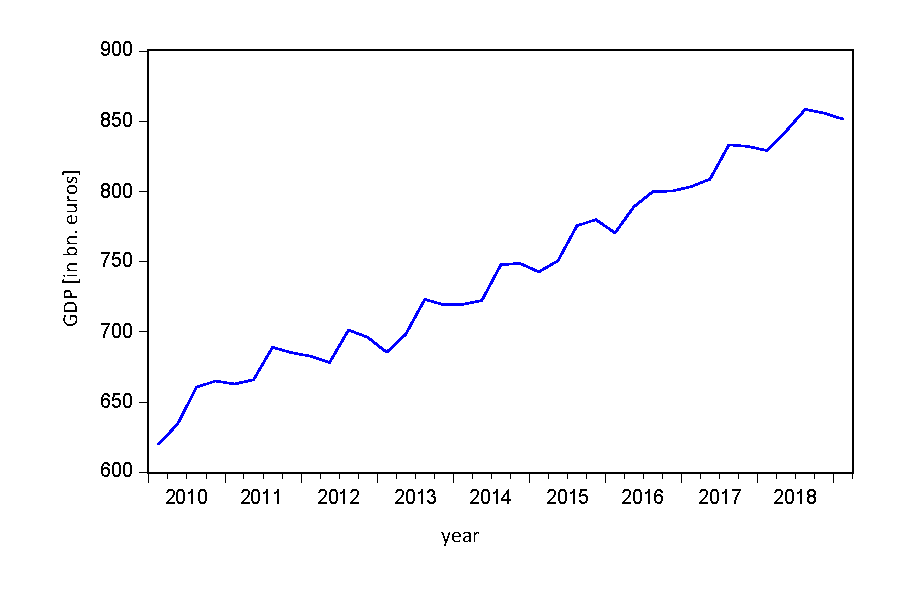
\includegraphics[width=12cm]{bip_de.pdf} %Width of the image and name of the file
	\caption{Gross domestic product of Germany at current prices, in billions of euros} %Figure caption
	\label{bip_de} %Reference for the text (see below)
	\end{center}
	\end{figure}
	
	Figure \ref{bip_de} describes \lipsum[1]
	
	\subsection{Two figures next to each other}
	
	% set two images next to each other:
	
	\begin{figure}[h]
		\centering
		\begin{minipage}[t]{0.45\linewidth}
			\centering
			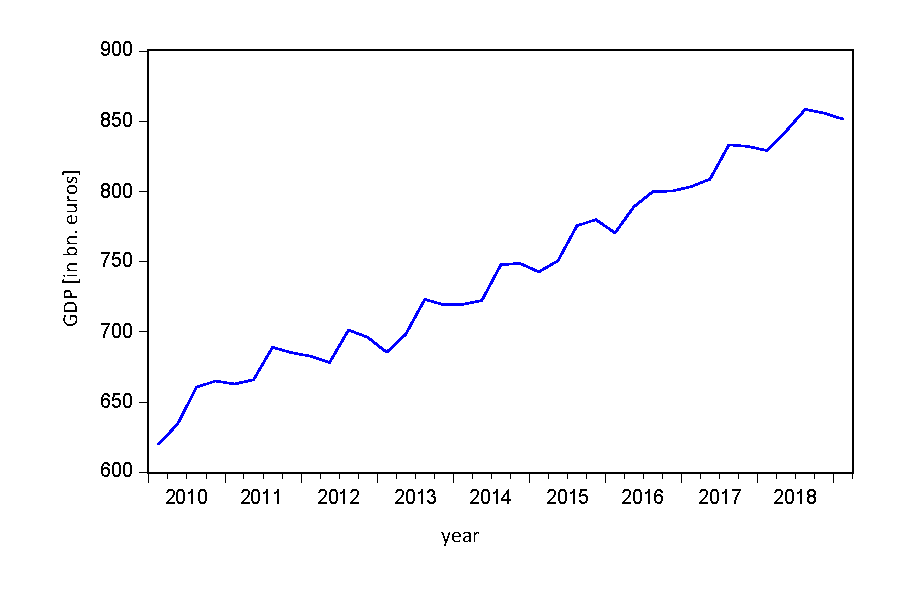
\includegraphics[width=8cm]{bip_de.pdf} %Width of the image and name of the file
			\caption{Test figure caption 1} %Figure caption
			%\label{Abbildungsverzeichnis}
			\label{test1}
		\end{minipage}
		\hfill
		\begin{minipage}[t]{0.45\linewidth}
			\centering
			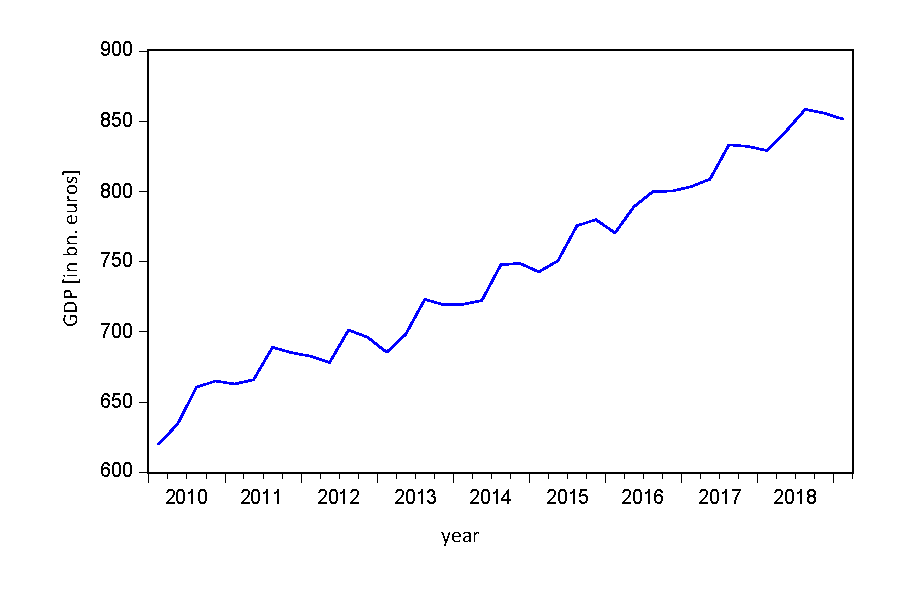
\includegraphics[width=8cm]{bip_de.pdf} %Width of the image and name of the file
			\caption{Test figure caption 2} %Figure caption
			%\label{Abbildungsverzeichnis}
			\label{test2}
		\end{minipage}
	\end{figure}
	Figure \ref{test1} and Figure \ref{test2} \lipsum[1] \\Furthermore, Figure \ref{bip_de} \lipsum[1]
	
	\section{Inserting tables}
	
	\begin{table}[h]
		\begin{center} %if centered alignment is desired
			\begin{tabular} {|c|c|c|c|} %Table with four columns is created, the text is centered and the columns are separated by vertical lines
				\hline %horizontal line is generated (to separate the rows)
				Column heading 1 & Column heading 2 & Column heading 3 & Column heading 4 \\ \hline
				example text & example text & example text & example text \\ \hline
				example text & example text & example text & example text  \\ \hline
				example text & example text & example text & example text  \\ \cline{2-3} %horizontal line is only generated for cells of column 2 to 3
				example text & example text & example text & example text  \\ \hline
				example text & example text & example text & example text  \\ \hline \hline
				example text & example text & example text & example text \\ \hline
			\end{tabular}
		\end{center}
		\caption{Example table} %Table caption
		\label{tab_a}
	\end{table}
	
	
	Table \ref{tab_a} describes...
	
	\clearpage
	\addcontentsline{toc}{section}{Appendix} 					%sets header with chapter title
	
	\section*{Appendix}
	\markright{Appendix}
	
	
	
	\clearpage
	\addcontentsline{toc}{section}{Bibliography} 	%sets header with chapter title
	\printbibliography
	
	
	\clearpage
	\section*{Declaration of originality}
	\thispagestyle{empty}
	I hereby declare that I have written this Bachelor Thesis independently and without using other than the indicated sources and aids and that I have identified the passages taken verbatim or in content from the used sources as such. The work in the same or similar form has not been submitted to any other examination authority.
	\\[1cm]
	CITY, DD.MM.YYYY
	\\[1.5cm]
	MARTINA MUSTERMANN
	
\end{document}
